\documentclass{article}

\usepackage{epsfig}
\usepackage{graphics}

\setlength{\textheight}{23.5cm}
\setlength{\topmargin}{-1cm}
\setlength{\textwidth}{155mm}
\setlength{\oddsidemargin}{2mm}

\title{DGtal: Digital  Geometry Tools and Algorithms Library}
\author{David Coeurjolly$^1$ \qquad \qquad Jacques-Olivier Lachaud$^2$ \\
  (For the DGtal Team)\\
${}^1$ LIRIS (UMR CNRS 5205), Universit\'{e} de Lyon, F-69622 \\
${}^2$ LAMA (UMR CNRS 5127), Universit\'{e} de Savoie, F-73376\\
}
\date{}

%%% -----------------------------
%%% Demonstration submission form:
%%% Title: DGtal: Digital Geometry Tools and Algorithms
%%% Authors:
%%% Institution:
%%% Content already published: YES/NO (If yes, please precise the conference/journal)
%%% Abstract:  (you can attach to the mail a pdf file including images/text)

% Guillaume Damiand\inst{1} Bertrand Kerautret\inst{2} \and Jacques-Olivier Lachaud\inst{2} Tristan Roussillon\inst{1} \and }

\begin{document}

\maketitle

DGtal is a generic open source library for Digital Geometry
programming whose main objective is to gather and structure different
developments from the digital geometry and topology community. The
benefits are numerous: to make easier the appropriation of our tools
for a neophyte (new PhD students, researchers from other topics,
\ldots), to permit better comparisons of new methods with already
existing approaches, to construct a federative project. Furthermore we
believe this is a necessary step for a better recognition of the
efficiency of discrete geometry techniques by the important image
analysis community. As a consequence, DGtal is designed so as to
simplify the construction of effective demonstration tools. New
results are thus easily shared to a vast audience. 

On a more technical level, DGtal is developed in C++. Similarly to
other classical libraries such as CGAL, it follows the paradigm of
genericity with efficiency. This approach is made possible with the
now well-known notion of concepts, implemented with templated
types. The kernel of DGtal offers digital spaces of arbitrary
dimension, with user-chosen integer types. Several digital topology
algorithms are already implemented (Rosenfeld topology, connected
components, simple points, homotopic thinning). The kernel manages
generic images (standard raster images but also tree images), and
arbitrary file formats with ImageMagick installed. Basic geometric
primitives (digital lines and segments) are also available, as well as
arbitrary dimensional volumetric distance transforms. A stream
mechanism has been developed to display digital objects and export
results in different vector formats.

DGtal is a collaborative effort --- for now --- of the French digital
geometry community. It is still a work of progress but show already
many promises to be the common basis for future developments made by
the digital geometry community. The next milestone (DGCI) should
include grid topology, geometric primitives and estimators, and other
elements. Visit the DGtal home page: \texttt{http://liris.cnrs.fr/dgtal}.

Main participants: D. Coeurjolly (LIRIS, Lyon), G. Damiand (LIRIS,
Lyon), S. Fourey (GREYC, Caen), B. Kerautret (LORIA, Nancy),
J.-O. Lachaud (LAMA, Chambéry), L. Provot (LORIA, Nancy),
T. Roussillon (LIRIS, Lyon), I. Sivignon (Gipsa-lab, Grenoble).

\begin{figure}
  \begin{center}
    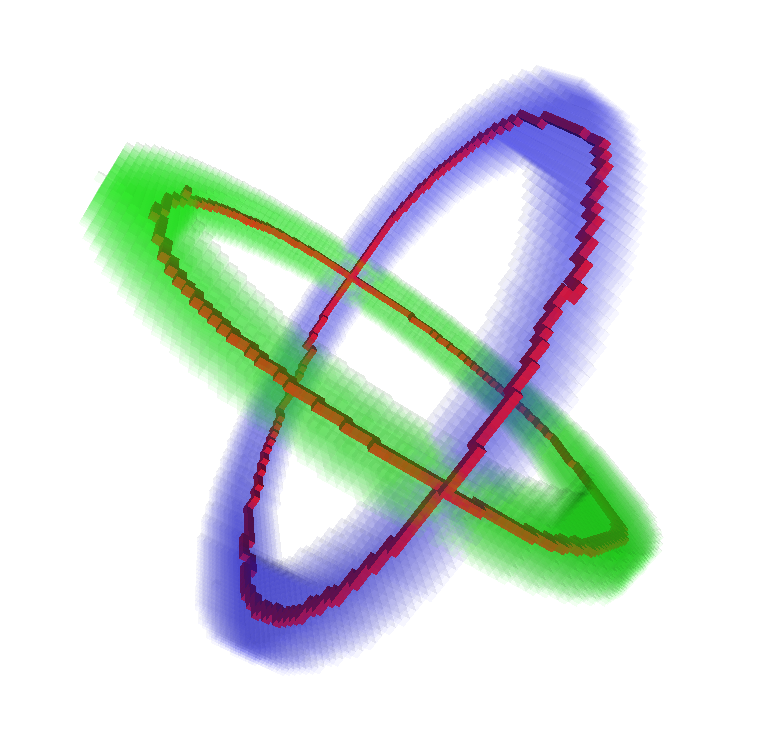
\includegraphics[width=0.24\textwidth]{./thinning-3D}
    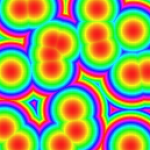
\includegraphics[width=0.24\textwidth]{./edt-2D}
    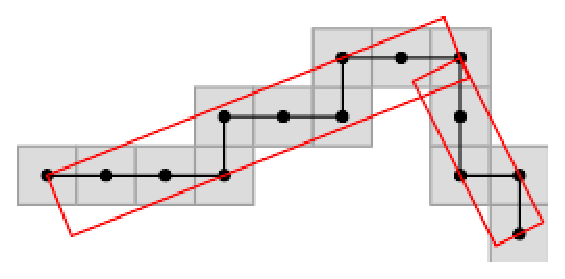
\includegraphics[width=0.24\textwidth]{./dss}
    \includegraphics[width=0.24\textwidth]{./hashtree}
  \end{center}
  
  \caption{(a) 3D homotopic thinning. (b) 2D euclidean distance transform. (c) Digital straight segment decomposition. (d) 2D image with a pointerless quadtree.}
\end{figure}

\end{document}
